%%%%%%%%%%%%%%%%%%%%%%%%%%%%%%%%%%%%%%%%%%%%%%%%%%%%%%%
%% Bachelor's & Master's Thesis Template             %%
%% Copyleft by Artur M. Brodzki & Piotr Woźniak      %%
%% Faculty of Electronics and Information Technology %%
%% Warsaw University of Technology, 2019-2020        %%
%%%%%%%%%%%%%%%%%%%%%%%%%%%%%%%%%%%%%%%%%%%%%%%%%%%%%%%

\documentclass[
    left=2.5cm,         % Sadly, generic margin parameter 
    right=2.5cm,        % doesnt't work, as it is
    top=2.5cm,          % superseded by more specific
    bottom=3cm,         % left...bottom parameters.
    bindingoffset=6mm,  % Optional binding offset.
    nohyphenation=false % You may turn off hyphenation, if don't like.
]{eiti/eiti-thesis}

\langpol % Dla języka angielskiego mamy \langeng
\graphicspath{{img/}}             % Katalog z obrazkami.
\addbibresource{bibliografia.bib} % Plik .bib z bibliografią
\usepackage{listings}

\begin{document}

%--------------------------------------
% Strona tytułowa
%--------------------------------------
\MasterThesis % Dla pracy inżynierskiej mamy \EngineerThesis
\instytut{Informatyki}
\kierunek{Informatyka}
\specjalnosc{Sztuczna inteligencja}
\title{
Kompilacja przez interpretację:\\
statyczne metaprogramowanie w języku C-=-1
}
\engtitle{ % Tytuł po angielsku do angielskiego streszczenia
    Unnecessarily long and complicated thesis' title \\
    difficult to read, understand and pronounce
}
\author{Adam Grabski}
\album{283431}
\promotor{dr. hab. inż. Ilona Bluemke}
\date{\the\year}
\maketitle

%--------------------------------------
% Streszczenie po polsku
%--------------------------------------
\cleardoublepage % Zaczynamy od nieparzystej strony
\streszczenie 
Statyczne metaprogramowanie jest nowym i dynamicznie rozwijającym się trendem w językach niskiego poziomu.
Wszystkie tego typu mechanizmy, niosą ze sobą jednak poważne ograniczenia.
C-=-1 proponuje nowe podejście do konstrukcji kompilatora, umożliwiające wprowadzenie do języka bardzo potężnych mechanizmów metaprogramistycznych. 
\slowakluczowe XXX, XXX, XXX

%--------------------------------------
% Streszczenie po angielsku
%--------------------------------------
\newpage
\abstract \kant[1-3]
\keywords Metaprogramowanie, XXX, XXX

%--------------------------------------
% Oświadczenie o autorstwie
%--------------------------------------
\cleardoublepage  % Zaczynamy od nieparzystej strony
\pagestyle{plain}
\makeauthorship

%--------------------------------------
% Spis treści
%--------------------------------------
\cleardoublepage % Zaczynamy od nieparzystej strony
\tableofcontents

%--------------------------------------
% Rozdziały
%--------------------------------------
\cleardoublepage % Zaczynamy od nieparzystej strony
\pagestyle{headings}

\section{Wstęp}
Celem tej pracy jest zaproponowanie nowych mechanizmów statycznego 
metaprogramowania.
Zostały one zaprojektowane z myślą o statycznej analizie kodu oraz prostocie projektowania nowych analizatorów.
Statyczna analiza kodu to technika wyciągania wniosków na temat programu, na podstawie wyłącznie jego kodu źródłowego \cite{survey_of_metaprograming}.

Jednym z ważniejszych celów analizatora jest wykrywanie typowych błędów programistycznych, bez uruchomienia programu.
Ostatnia dekada rozwoju języków programowania i narzędzi z nimi związanych wskazuje, że zapotrzebowanie na statyczną analizę kodu rośnie.
W tym samym czasie doszło do gwałtownego wzrostu zainteresowania metaprogramowaniem. Ten termin obejmuje zarówno refleksję, czyli pozyskiwanie informacji o strukturze programu, jak i modyfikację kodu. W zależności od tego, czy dany mechanizm jest aktywny w czasie kompilacji, czy uruchomienia, nazywamy go odpowiednio statycznym lub dynamicznym.
Meta-program można zdefiniować jako aplikację, która spełnia jedno z następujących wymagań \cite{nielson2004principles}:
\begin{enumerate}
\item Program operuje na innym programie.
\item Program wytwarza inny program jako swój wynik.
\item Program uzyskuje dostęp lub modyfikuje własną strukturę.
\end{enumerate}

Zaproponowane w tej pracy mechanizmy, opisane dokładniej w rozdziale \ref{Attributes_definition}, umożliwiają stworzenie aplikacji jawnie złożonej z dwóch części:
konwencjonalnego programu, który zostanie skompilowany do formy wykonywalnej oraz meta-programu, który zostanie wykonany w czasie kompilacji.
Celem meta-kodu jest wykonanie analizy oraz modyfikacji konwencjonalnej części aplikacji.
Aby to osiągnąć, zaprojektowany został nowy, uproszczony język programowania zawierający proponowane mechanizmy.
Nie użyto istniejącego języka, aby ułatwić stworzenie kompilatora.

Kontynuując tradycję zaczętą przez Bjarne Stroustrup-a nazwa, którą nadano temu nowemu językowi, jest żartem programistycznym. C++ swoją nazwę wziął od jednego ze sposobów na inkrementację zmiennej o nazwie C \cite{stroustrup_com}. 
W ten sam sposób, w który C++ jest rozwiniętą wersją C, C-=-1 (wymawiane 'cm1') jest nietypową alternatywą dla C++. C-=-1 zostało nazwane na podstawie C++ ponieważ dzieli z nim podstawy filozoficzne oraz niektóre decyzje projektowe. Te podobieństwa zostały opisane w rozdziale 3.
W ramach prac badawczych zaimplementowano podstawową bibliotekę standardową oraz napisano szereg prostych programów z jej wykorzystaniem. Następnie porównano je z programami, osiągającymi ten sam cel, napisanymi w innych językach programowania, pod kątem złożoności, czytelności i powstałych plików wykonywalnych.
         % Wygodnie jest trzymać każdy rozdział w osobnym pliku.
\section{Istniejące rozwiązania}

Wśród przemysłowo stosowanych języków programowania istnieje szeroka gama mechanizmów metaprogramistycznych. Stosuje się w nich zarówno statyczną, jak i dynamiczną refleksję. 
W popularnie używanych językach mechanizmy dynamiczne są zwykle dużo bardziej rozbudowane i przyjazne użytkownikowi.

W tym rozdziale zostaną przedstawione wybrane języki programowania oraz dostępne w nich mechanizmy metaprogramistyczne.
Te istniejące rozwiązania będą stanowić podstawę dla analizy możliwości C-=-1.



\subsection{C\#}
Język C\# od początku swojego istnienia wspierał refleksję\cite{csharp:getType}.
Środowisko uruchomieniowe DotNet zostało zaprojektowane z myślą o dynamicznym ładowaniu plików bibliotecznych \cite{csharp:assemblies}.
W związku z tym większość mechanizmów metaprogramistycznych w językach opartych na nim jest używana w trakcie uruchomienia.
W ostatnich wersjach Microsoft dodał jednak pewne możliwości do generowania i analizowania kodu w trakcie kompilacji, w ramach otwartego kompilatora Roslyn \cite{csharp:source_generators}.

\subsubsection{Atrybuty}
W języku C\# atrybuty służą głównie do przechowywania metadanych \cite{csharp:attributes}.
Na rynku, istnieją rozwiązania, które wykorzystują takie adnotacje do modyfikacji programu, jednak takie zastosowanie nie jest proste.
Ponadto, jakiekolwiek zmiany w kodzie aplikacji, będą zachodzić w trakcie uruchomienia, nie kompilacji.
Oznacza to narzuty, zarówno czasu wykonania, jak i wielkości pliku wykonywalnego, które w wielu kontekstach są nieakceptowalne \cite{csharp:reflection_cost, cpp:reflection:high_performance}.
\subsubsection{Refleksja}

Informacja o organizacji programu jest integralną częścią skompilowanego pliku C\#.
W czasie uruchomienia aplikacja ma pełny wgląd we własną strukturę.
Ponieważ w C\# występuje dynamiczna refleksja, program ma również dostęp do metadanych w bibliotekach ładowanych w czasie pracy.
Ten mechanizm niesie ze sobą też pewne koszty.
Refleksja w czasie uruchomienia niesie za sobą poważne koszty, które w niektórych kontekstach są nieakceptowalne.
Ponadto, obecność informacji o typach i funkcjach w skompilowanym pliku znacząco ułatwia dekompilację.

Można też argumentować, że dostęp do metadanych programu w trakcie uruchomienia utrudnia optymalizacje.
Program może przeglądać własną strukturę i dynamiczne wywoływać kod na podstawie pozyskanych informacji.
W związku z tym niektóre typy optymalizacji takie jak \lstinline{inlining} (bezpośrednie użycie ciała funkcji, zamiast jej wywołania) nie są możliwe \cite{dotnet:method_inlining}.

\subsubsection{Analizatory kodu}

Jednym z wyników publicznego udostępnienia kodu kompilatora Roslyn\cite{roslyn}, było udostępnienie programistom API kompilatora służącego do analizy kodu.
Programista może więc stworzyć własny analizator w ramach swojego projektu.
Zaletą tego podejścia  jest spójność używanego języka.
Projekt pisany w C\# może być analizowany w C\#, bez żadnych dodatkowych restrykcji.
Unika to problemu tworzenia dodatkowego dialektu języka, jaki występuje w C++.

\subsubsection{Generatory kodu}

Kompilator Roslyn w języku C\#9 wprowadził również, możliwość pisania generatorów kodu \cite{csharp:source_generators,roslyn}.
Jest to bardzo podobne rozwiązanie do makr w języku Rust \cite{rust, klabnik2019rust}. Generatory kodu to specjalne klasy, których kod jest wykonywany w trakcie kompilacji. 
Mechanizm C\# jest jednak bardziej zaawansowany.
Umożliwia generowanie kodu, używając wszystkich elementów języka, zamiast zapewniać prosty szablon.
Te generatory, tak jak w Rust, nie mają jednak dostępu do informacji zbieranych przez kompilator, poza drzewem składniowym oraz nie mogą modyfikować istniejącego kodu.

Generatory kodu nadal są rozwijane i stanowią już część stabilnego C\#.
Stanowią one jednak ciekawą zmianę w kierunku rozwoju języka. 
Generatory kodu są pierwszym przejawem statycznego metaprogramowania w C\#

\subsection {Rust}
Ponieważ Rust \cite{rust, klabnik2019rust} jest stosunkowo młody, jego projektanci mogli czerpać z doświadczeń innych języków. Wyraźnie widać to w jego składni, zintegrowanym systemie zarządzania zależnościami oraz bardzo przyjaznym kompilatorze.\par
Z tego powodu, nie zawiera on też tradycyjnego preprocesora, takiego jak w C/C++ czy C\#. Makra w Rust są tak naprawdę funkcjami operującymi na drzewie składniowym programu. Jest to zdecydowany postęp względem prostego zastępowania tekstu jak w C/C++, lecz ma też swoje wady.\par
Makra w języku Rust nadal operują na, co prawda strukturyzowanym, ale nadal, tekście. Oznacza to, że nie mają one dostępu do systemu typów ani żadnych innych informacji zgromadzonych przez kompilator.\par
\subsection{C++20}
C++ \cite{ISO:cpp20} zawiera szeroką gamę mechanizmów metaprogramistycznych oraz technik do statycznej analizy kodu. Były one stopniowo wprowadzane do języka przez cały czas jego istnienia, bez spójnego planu.\par
\subsubsection{Szablony}
Szablony w C++ można rozumieć jako oddzielny, funkcyjny, zdolny do symulacji maszyny Turinga \cite{template_turing_complete}, język programowania.
Metaprogramowanie szablonowe powstało nie jako świadomy wysiłek twórców języka, lecz jako naturalna, nieprzewidziana konsekwencja jego zasad.

\subsubsection{Koncepty}
Koncepty (ang: concept) zostały wprowadzone w C++20 \cite{ISO:cpp20} jako sposób na lepsze dokumentowanie szablonów oraz czytelniejsze komunikaty o błędzie w wypadku niepoprawnego użycia.
Używa się ich do ograniczania, które typy mogą zostać wykorzystane w danym szablonie.
Stanowią praktyczną aplikację idei ograniczonego polimorfizmu z teorii typów \cite{Cardelli85onunderstanding}.

Koncepty są definiowane jako zbiór wymagań, które typ musi spełnić.
Mogą to być proste wyrażenia logiczne, jak i weryfikowanie czy dana metoda istnieje oraz jaki typ zwraca.
W przeciwieństwie do pozostałych omawianych mechanizmów koncepty bronią programistę przed niezrozumiałymi błędami kompilacji zamiast przed błędami wykonania.

\subsubsection{Atrybuty}
Atrybuty zostały oficjalnie wprowadzone do języka w C++11\cite{ISO:2012:III}. 
Umożliwiają one przekazanie kompilatorowi dodatkowych informacji na temat kodu źródłowego.
Te dane są potem wykorzystywane w trakcie kompilacji do wydawania lub ignorowania ostrzeżeń.
Dwa przykłady warte omówienia to \lstinline{fallthrough} oraz \lstinline{no_discard}, ponieważ prezentują obydwa przypadki zastosowania atrybutu.

Atrybut \lstinline{fallthrough} powstał, aby rozwiązać typowy problem języków zawierających konstrukcję \lstinline{switch}. W większości zastosowań celem programisty jest stworzenie zestawu niezależnych od siebie przypadków, spośród których zostanie wykonany jeden na podstawie wartości jakiejś zmiennej.\par
Niestety domyślnym zachowaniem konstrukcji \lstinline{switch}, po wykonaniu bloku jest przejście do następnego (tak zwany \lstinline{fallthrough}). Kompilatory zaczęły więc wydawać ostrzeżenie, jeśli blok case nie zostanie zakończony instrukcją \lstinline{break}. To tworzy jednak inny problem: czasami programista chce osiągnąć dokładnie takie zachowanie. Niektóre kompilatory zaczęły przez to zwracać uwagę na komentarze, szukając tam wyrażenia \lstinline{fallthrough} (w GCC flaga -Wimplicit-fallthrough=3) \cite{gcc_warnings}.\par
W C++11 sformalizowano to zachowanie, tworząc atrybut \lstinline{fallthrough} \cite{ISO:2012:III}. Zaaplikowanie go do przypadku konstrukcji \lstinline{switch}, powstrzymuje kompilator przed wydaniem ostrzeżenia.\par
Atrybut \lstinline{no_discard}, zamiast uciszać ostrzeżenie, generuje je. Jego zadaniem jest wykrywanie sytuacji, w których programista ignoruje wartość zwracaną przez funkcję. Można go zaaplikować zarówno do typów (wtedy każda funkcja zwracająca ten typ staje się \lstinline{no_discard}) lub do funkcji.\par
Typowym przykładem zastosowania tego atrybutu są kody błędów. Ze względu na duży koszt mechanizmu wyjątków w C++, w niektórych projektach się ich nie stosuje. Zamiast tego, funkcje których wykonanie może się nie powieść, zwracają strukturę informującą o błędzie. Ponieważ programista wywołujący taką funkcję, nie ma obowiązku sprawdzić wyniku tego wywołania, łatwo było o błąd. Stąd konieczność atrybutu \lstinline{no_discard}.

Podstawową wadą atrybutów w C++ jest fakt, że są one zachowaniem bezpośrednio wpisanym w kompilator. Nie istnieje możliwość napisania własnego atrybutu a ich lista, jest bardzo krótka.\par
\subsubsection{Funkcje constexpr}
Język C++11 wprowadził koncepcję \lstinline{constexpr}\cite{ISO:2012:III}.
Zaaplikowanie tego modyfikatora do zmiennej lub funkcji, informuje kompilator, że mogą one być ewaluowane w trakcie kompilacji. Funkcje \lstinline{constexpr} mają też nałożony szereg ograniczeń co do swojej struktury. Z każdą kolejną wersją języka jest ich coraz mniej, jednak nie każda funkcja może być ewaluowana w trakcie kompilacji.

Ponadto, funkcje \lstinline{constexpr} nie mają większego dostępu do struktury programu niż normalny program. Nie dają one możliwości modyfikowania istniejącego ani generowania nowego kodu. Stanowią one więc jedynie sposób na optymalizację programu.
W związku z tym mechanizm \lstinline{constexpr} został skrytykowany za jawne definiowanie które funkcje są wykonywalne w czasie kompilacji.
Yauhen Klimiankou argumentował \cite{Klimiankou:contexpr_great_good_wrong_idea}, że wykonywalność funkcji w czasie kompilacji powinna być przejrzysta dla programisty i obsługiwana przez kompilator automatycznie.
    % Umożliwia to również łatwą migrację do nowej wersji szablonu:
\section{Projekt języka}
\label{Language_desig}
%todo: talk about limitations on interpreting and compilation, which functions can be executed, when
Język C-=-1 w przeciwieństwie do większości współczesnych języków programowania jest oparty na udostępnieniu programiście struktur danych tworzonych przez kompilator. Deskryptory typów, funkcji, przestrzeni nazw oraz enumeratorów, razem z reprezentacją pośrednią kodu są udokumentowaną częścią języka (załącznik nr 1).
Aby umożliwić użytkownikowi wykorzystanie tych struktur danych, C-=-1 musi zapewnić sposób na napisanie kodu wykonywanego w czasie kompilacji, który może nimi manipulować. W tym celu postanowiono rozszerzyć koncepcję atrybutu, aby umożliwić inspekcję i modyfikację reprezentacji pośredniej.
C-=-1 został zaprojektowany na bazie założeń C++. Obydwa te języki są statycznie typowane, kompilowane oraz nie wymagają specjalnego środowiska uruchomieniowego.
Przy projektowaniu C-=-1 skorzystano jednak z doświadczeń wyciągniętych z C++ w aspektach takich jak dziedziczenie wielobazowe czy zarządzanie pamięcią. Obydwa zostały opisane odpowiednio w rozdziałach \ref{elementy_jezyka} oraz \ref{struktura_paczki}

\subsection{Składnia}

\subsection{Elementy języka}
\label{elementy_jezyka}

\subsubsection{Klasy}
\label{classes_definition}
Klasy w języku C-=-1 działają analogicznie do języków z rodziny C.
Są to zbiory danych (pola klasy) z którymi powiązane są pewne operacje (metody).
Wszystkie elementy takiego typu mogą mieć ograniczenia dostępu.
Dwoma istotnymi elementami klas w C-=-1 są metody specjalne \lstinline{construct} oraz \lstinline{finalize}.
Można je zrozumieć jako odpowiedniki konstruktora oraz destruktora z C++.
Ponieważ C-=-1 w swojej obecnej formie nie wspiera wyjątków, nie gwarantuje wykonania finalizatorów zmiennych lokalnych w wypadku nieoczekiwanego zakończenia programu.

%todo: reference this
\begin{minipage}{\linewidth}
  
	\begin{lstlisting}[
	  numbers=left,
	  firstnumber=0,
	  caption={Fragment gramatyki C-=-1 deklarujący klasę},
	  aboveskip=0pt,
	  label={lst:class_grammar}
	  ]
typeDeclaration:
(attributeSequence)? AccessSpecifier? classTypeSpecifier identifier 
  genericSpecifier? (
  ':' implementedInterfacesSequence
  )? '{' classContentSequence '}';
classTypeSpecifier: ('class' | 'interface' | 'struct');
  \end{lstlisting}
  \end{minipage}

\subsubsection{Interfejsy}
\subsubsection{Funkcje}
W C-=-1 funkcje oraz metody działają na tej samej zasadzie co w C++.
Istotną różnicą jest możliwość ich wykonania w czasie kompilacji.
Domyślnie, funkcje mogą być wykonywane w dowolnym kontekście.
O ile programista nie sprecyzował żadnych ograniczeń, podprogram może zostać wykonany zarówno w czasie uruchomienia, jak i kompilacji.
Wywoływanie funkcji w trakcie kompilacji ma kilka różnych zastosowań.

Optymalizacja programu, historycznie stanowiła podstawową motywację dla wykonywania kodu w czasie kompilacji.
Jeśli wyrażenie zależy wyłącznie od stałych, kompilator może podjąć decyzję o jego ewaluacji do stałej.
C-=-1, w przeciwieństwie do C++, umożliwia optymalizację niemalże dowolnej funkcji w ten sposób.
Ponieważ programista nie musi jawnie precyzować, że procedura jest wykonywalna w czasie kompilacji, język C-=-1 unika problemów powiązanych z modyfikatorem \lstinline{constexpr} z C++ \cite{Klimiankou:contexpr_great_good_wrong_idea}
Taka możliwość tworzy także pewne wyzwania, dokładniej opisane w rozdziale \ref{compile_time_constant_evaluation}.

\subsubsection{Atrybuty}
\label{Attributes_definition}

Atrybuty stanowią najważniejszy aspekt C-=-1.
To za ich pomocą, programista ma dostęp do wszystkich mechanizmów metaprogramistycznych, będących tematem tej pracy.
Możliwości, które atrybuty oferują, są dokładniej opisane w rozdziale \ref{Attributes_mechanism_cm1}.

Atrybuty są bardzo zbliżone do klas: składają się z metod, pól oraz konstruktorów i mogą implementować interfejsy.
Podobieństwa te kończą się jednak na najbardziej podstawowych tych bytów.
Klasy i atrybuty pełnią w C-=-1 diametralnie różne role i istnieją w odrębnych kontekstach.
Atrybuty mogą być tworzone wyłącznie jako adnotacje do innych elementów programu, a ich instancje istnieją wyłącznie w czasie kompilacji.

Listing \ref{lst:attribute_basic_example} zawiera przykład prostego atrybutu w C-=-1.
Składniowo ta deklaracja jest niemalże identyczna, do deklaracji klasy opisanej w rozdziale \ref{classes_definition}.
Największą różnicą jest użycie słowa kluczowego \lstinline{att} i deklaracja celu atrybutu, zamiast \lstinline{class}.

\begin{minipage}{\linewidth}
  
	\begin{lstlisting}[
	  numbers=left,
	  firstnumber=0,
	  caption={Fragment gramatyki C-=-1 deklarujący atrybut},
	  aboveskip=0pt,
	  label={lst:attribute_grammar}
	  ]
attributeDeclaration: 
  (AccessSpecifier)? 'att' '<' attributeTarget+ '>' 
  identifier (':' implementedInterfacesSequence)?
  '{' classContentSequence '}';

attributeTarget: ('type' | 'variable' | 'function');
  \end{lstlisting}
  \end{minipage}

Listing \ref{lst:attribute_grammar} zawiera fragment gramatyki C-=-1, w notacji EBNF \cite{ebnf}.
Wyraźnie widać w niej podobieństwo do deklaracji klasy z listingu \ref{lst:class_grammar}.
Ciało atrybutu używa wręcz tej samej reguły co ciało klasy.
Istotnym elementem gramatyki atrybutu, jest natomiast wspomniany wcześniej cel atrybutu (reguła \lstinline{attributeTarget}), deklarujący, do których elementów języka można przyłączyć dany atrybut.

W obecnym stanie języka istnieją trzy cele: funkcje, zmienne i typy, zgodnie z linią piątą listingu \ref{lst:attribute_grammar}.
Atrybut może być powiązany z wieloma celami.
W zależności od obsługiwanych celów atrybut ma do zaimplementowania różny zestaw metod, reagujący na użycie danego elementu modelu semantycznego (rozdział \ref{implementation:intermidiate_representation}).
Przykładowo dla funkcji, te metody to między innymi \lstinline{onCall}, powiązana z wywołaniem procedury.
Wszystkie atrybuty mają również metodę \lstinline{attach}, wywoływaną po stworzeniu nagłówka elementu modelu.
Te funkcje zostały opisane w rozdziale \ref{Attributes_mechanism_cm1}.

\begin{minipage}{\linewidth}
  
	\begin{lstlisting}[
	  numbers=left,
	  firstnumber=0,
	  caption={Przykład atrybutu w C-=-1},
	  aboveskip=0pt,
	  label={lst:attribute_basic_example}
	  ]
  public att<function> SomeAttribute
  {
	private _number: usize;
	public fn construct(number: usize)
	{
		self._number = number;
	}
	public fn attach(f: functionDescriptor)
	{}
  }
  \end{lstlisting}
  \end{minipage}
\subsection{Mechanizm atrybutów}
\label{Attributes_mechanism_cm1}

Celem istnienia atrybutów w C-=-1 jest: modyfikacja metadanych elementów programu oraz analiza i modyfikacja kodu.
Kompilator bezpośrednio wywołuje ich metody, jako część procesu kompilacji, co zostało oznaczone na rysunku \ref{compilation_process_diagram}.
W zależności od tego, które cele atrybut obsługuje, może zaimplementować różny zestaw funkcji specjalnych, opisanych w rozdziale \ref{design:attributes:special_functions}.

Istotnym ograniczeniem atrybutów C-=-1 jest brak możliwości użycia elementów biblioteki, w której zostały zdefiniowane.
To obostrzenie zostało wprowadzone, aby atrybuty można było aplikować wewnątrz tego samego projektu, oraz aby zapewnić większą deterministyczność kompilacji.
Rysunek \ref{design:attributes:attribute_function_dependendcy} zawiera diagram zależności w programie, którego działanie byłoby zależne od implementacji kompilatora.
\lstinline{Atrybut} modyfikuje kod funkcji, do której jest przyłączony.
Zarówno \lstinline{Funckja A}, jak i \lstinline{Funkcja B} są nim adnotowane.
\lstinline{Atrybut}, w trakcie modyfikowania kodu funkcji, wywołuje \lstinline{Funkcje A}.
W tej sytuacji, ciało \lstinline{Funkcji B} zależy od kolejności, w której operacje metaprogramistyczne będą wykonywane.
Jeśli kompilator najpierw weźmie pod uwagę \lstinline{Funkcje A}, zostanie ona zmodyfikowana, używając oryginalnej wersji \lstinline{Funkcji B}.
Oznacza to, że skutki zaaplikowania \lstinline{Atrybutu} zależą od implementacji kompilatora.
Ograniczenie na kodzie używalnym przez atrybut wynika też z funkcji specjalnej \lstinline{attach}.
Jest ona wykonywana, kiedy istnieje tylko nagłówek dołączonego obiektu.
W związku z tym kod atrybutu oraz wszystkie jego zależności muszą być skompletowane, zanim tworzenie reprezentacji pośredniej pakietu zostanie zakończone.

Usunięcie wymagania, aby atrybutami można było adnotować elementy tego samego pakietu, umożliwiłoby używanie funkcji w nim zdefiniowanych.
Nie podjęto jednak tej decyzji.
Najbardziej prawdopodobnym scenariuszem użycia atrybutów, jest tworzenie prostych analizatorów i metaprogramów powiązanych z domeną aplikacji, używając bibliotek przeznaczonych do analizy kodu.
Sytuacja, w której atrybut musi użyć kodu z pakietu, w którym jest zdefiniowany, jest mało prawdopodobna.

\begin{figure}
	\caption{Diagram ilustrujący przykładowe zależności między atrybutem a funkcjami}
	\label{design:attributes:attribute_function_dependendcy}
	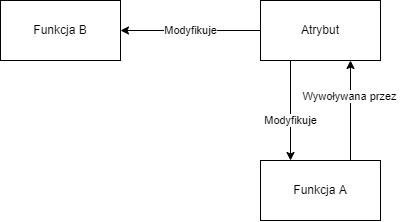
\includegraphics{attribute_function_dependency.png}
\end{figure}

\subsubsection{Funkcje specjalne}
\label{design:attributes:special_functions}

Funkcje specjalne atrybutów, służą do reagowania na użycie obiektu, z którym powiązana jest adnotacja.
Ma to ułatwić tworzenie analizatorów.
Tworząc na przykład odpowiednik niezmiennika \lstinline{const} z C++, programista musi znaleźć wszystkie użycia zmiennej.
W obecnej wersji C-=- istnieją następujące funkcję specjalne:
\begin{itemize}
	\item Funkcje\begin{itemize}
		\item \lstinline{onCall}
	\end{itemize}
	\item Zmienne\begin{itemize}
		\item \lstinline{onDeclare}
		\item \lstinline{onReference}
	\end{itemize}
\end{itemize}
%todo: more, this is an important part of the thesis
Ponadto, każdy cel ma ze sobą powiązaną funkcję \lstinline{attach}.
Ta procedura jest wywoływana, kiedy nagłówek obiektu został stworzony.
Na przykład dla funkcji, dzieje się to kiedy kompilator zebrał jej nazwę, parametry oraz typ zwracany.
Dzieje się to na etapie \lstinline{confirm} przetwarzania pliku źródłowego, który został dokładniej opisany w rozdziale \ref{implementation:source_processing_phases}.

Celem funkcji \lstinline{attach} jest modyfikowanie metadanych obiektu, zanim będą one potrzebne.
Ta procedura to jedyny czas, kiedy kod użytkownika może zmieniać dane używane przy wybieraniu przeciążenia funkcji.
To ograniczenie gra dużą rolę przy zapewnieniu deterministycznego wyniku kompilacji.
Proces wyboru przeciążenia funkcji w C-=-1, jest złożony i został dokładniej opisany w rozdziale \ref{Function_overload_resolution}.


\subsection{Reprezentacja pośrednia}\label{reprezentacja_posrednia}
Programista C-=-1 może analizować oraz modyfikować reprezentację pośrednią swojego programu w czasie kompilacji.
C-=-1 Intermidiate Representation, w skrócie CIR jest nieznacznie uproszczoną wersją języka, reprezentowaną jako struktura danych.
Użytkownik wchodzi w interakcje z CIR za pomocą zestawu interfejsów opisanych w załączniku 1.
Wszystkie typy instrukcji oraz wyrażeń mają ze sobą powiązany konkretny typ.
Wyjątkiem jest \lstinline{ScopeTerminationStatement}, który nie jest powiązany z żadną instrukcją pisaną przez użytkownika.
Instrukcja zakończenia zakresu jest wstawiana przez kompilator na koniec każdej instrukcji złożonej i jest odpowiedzialna za wywołanie destruktorów zmiennych lokalnych (opisane w rozdziale \ref{classes_definition}).

\begin{minipage}{\linewidth}
	\begin{lstlisting}[
		numbers=left,
		firstnumber=0,
		caption={Kod w C++ zawierający przeciążoną funkcję},
		aboveskip=0pt,
		label={lst:cpp_overloaded_function}
	]
int add(int a, int b);
float add(float a, float b);
int main() {
  add(1, 2);
  add(1.0, 2.0);
}
	\end{lstlisting}
\end{minipage}

CIR jest najbardziej zbliżona do drzewa AST programu.
Jednak, zamiast bazować na składni programu, ta struktura danych opiera się na jego semantyce.
Rozważmy fragment kodu C++ w listingu \ref{lst:cpp_overloaded_function}.
Zawiera on dwa przeciążenia funkcji \lstinline{add}: jedno przyjmujące dwa parametry \lstinline{int} a drugie przyjmujące \lstinline{float}.
Z punktu widzenia drzewa AST, wywołania w liniach 3 i 4, różnią się wyłącznie przekazywanymi stałymi.
Identyfikator funkcji (w tym wypadku \lstinline{add}) nie wskazuje jej w sposób unikatowy \cite{ISO:cpp20}, kompilator musi dokonać wyboru przeciążenia na podstawie przekazywanych parametrów \cite{cpp:function_overload_frontend}.

CIR, zamiast opierać się na tekście źródłowym, składa się z odniesień do konkretnych elementów programu.
Tak więc w kontekście przykładu z listingu \ref{lst:cpp_overloaded_function}, obiekty w modelu odpowiadające liniom 3 i 4 zawierałyby jednakowe wskazania na funkcje.
CIR, w przeciwieństwie do drzewa AST składa się więc wyłącznie z informacji o znaczeniu semantycznym, nie składniowym.

Przegląd literatury nie zawierał struktury danych o charakterystyce zbliżonej do CIR.
Zaproponowano więc nowy termin: reprezentacja semantyczna.
Opisuje on strukturę danych, opisującą program, składającą się wyłącznie z informacji o znaczeniu semantycznym.
Reprezentacja semantyczna zawiera komplet informacji potrzebnych do zrozumienia programu.
Operacje takie jak wybieranie przeciążenia, po jego skonstruowaniu, są zbędne.

\subsection{Zarządzanie pamięcią}
Zarządzanie pamięcią w C-=-1 jest oparte na C++11. W 2011 do biblioteki standardowej zostały wprowadzone nowe typy 'inteligentnych wskaźników': \lstinline{unique_ptr}, \lstinline{shared_ptr} oraz \lstinline{weak_ptr}\cite{ISO:2012:III}.
Miały one na celu wprowadzenie do języka mechanizmów umożliwiających tanie i automatyczne zarządzanie pamięcią oraz semantyczne podkreślenie relacji między obiektami.
Korzystając z doświadczeń C++, gdzie te wskazania stały się zalecanym sposobem zarządzania pamięcią\cite{cpp:core_guidelines}, inteligentne wskazania są integralną częścią C-=-1.
\subsection{Struktura pakietu}\label{struktura_paczki}
Projekt w języku C-=-1 jest identyfikowany przez plik manifestu (ang: manifest) o rozszerzeniu .mn. 
Zawiera on metadane na temat pakietu: unikatowy identyfikator, dane autora, zależności i tym podobne.
Pliki źródłowe mają rozszerzenia .cm. W tym samym folderze co manifest znajduje się folder \lstinline{src}. Kompilator zakłada, że wszystkie pliki o rozszerzeniu \lstinline{.cm} będące jego potomkami należą do projektu definiowanego przez manifest.
W pliku .mn zdefiniowane są metadane na temat pakietu takie jak autor, wersja czy zależności. Ten aspekt języka jest modelowany na bazie Rust i pliku \lstinline{cargo.toml}.
 % wystarczy podmienić swoje pliki main.tex i eiti-thesis.cls
\section{Implementacja}
W celu przeprowadzenia prac badawczych na temat konsekwencji zaproponowanych mechanizmów, koniecznym było zaimplementowanie podstawowego kompilatora. 
\subsection{Fazy kompilacji}
Ze względu na nietypową konstrukcję C-=-1, proces kompilacji musi być dłuższy oraz ostrożniej zaprojektowany niż w typowym statycznie typowanym języku programowania.
Ponieważ użytkownik ma pisać kod, który będzie modyfikował wewnętrzne struktury danych kompilatora, musi on wiedzieć kiedy które jej elementy są gotowe.
Kolejność operacji wykonywanych przez kompilator, staje się przez to częścią języka.
\begin{enumerate}
    \item Budowa reprezentacji pośredniej atrybutów
    \item Zebranie definicji funkcji i typów
    \item Przyłączenie atrybutów
    \item Budowa reprezentacji pośredniej funkcji i typów
    \item Wykonanie meta-funkcji atrybutów
    \item Zastąpienie wyrażeń zawierających statyczną refleksję ich wynikami
    \item Zapisanie reprezentacji pośredniej paczki
    \item (opcjonalne) Konwersja do postaci pośredniej LLVM i kompilacja do kodu maszynowego
\end{enumerate}

Współczesne kompilatory są typowo skonstruowane z trzech części: front-end, middle-end i back-end [9].
Zadaniem front-endu jest walidacja składni, weryfikacja typów oraz buduje reprezentację pośrednią kodu. Middle-end, operując na tych strukturach danych dokonuje optymalizacji niezależnych od maszyny docelowej.
Na koniec back-end optymalizuje kod pod kątem konkretnej architektury procesora i generuje kod maszynowy.

Ze względu na nietypowe wymagania C-=-1, zastosowano nowy podział odpowiedzialności.
W przeciwieństwie do typowych języków programowania, implementowany kompilator nie może wygenerować reprezentacji pośredniej programu jako jeden krok.
Punkt 3 procesu kompilacji, może wpływać na wybór rozwiązywanie przeciążeń funkcji.

Kompilator C-=-1 dzieli się na następujące części:
\begin{enumerate}
    \item Frontend
    \item Interpreter
    \item Optimiser
    \item Serialisator
    \item Backend Interface
    \item Backend
\end{enumerate}
Część z tych komponentów nazywa się tak samo jak w klasycznej architekturze. Jest to zabieg celowy, ponieważ pełnią one te same funkcje. Dodatkowe komponenty kompilatora które zostały wydzielone to: Interpreter, Serialisator oraz Backend Interface. Nazwa Optimiser została wybrana ponieważ wyrażenie „middle-end” rzadko występuje w literaturze a wybrany termin jest bardziej deskryptywny.

Ponieważ częścią kontraktu pomiędzy programistą a językiem C-=-1 jest kod wykonywany w czasie kompilacji, jednym z wydzielonych komponentów jest Interpreter. Operuje on na CIR omówionej w rozdziale 3.4. Interpreter stanowi najważniejszy komponent kompilatora, ponieważ większość transformacji odbywa się za jego pomocą. Szczegółowe działanie tego komponentu jest opisane w rozdziale 4.3.

Optimiser został dodany do struktury kompilatora, aby zapewnić możliwość dalszego rozwoju i dla kompletności projektu. Nie został jednak zaimplementowany.

Serializator jest odpowiedzialny za zapisywanie i odczytywanie struktur danych kompilatora z formy tekstowej. Służy to zarządzaniu zależnościami. Zserializowaną w ten sposób paczkę można dystrybuować za pomocą serwisu takiego jak NPM oraz używać w innych projektach. Ponieważ zawartością takiego modułu jest zserializowane, niezależne od platformy CIR, nie istnieje problem binarnej kompatybilności. Kompilacja programu używając paczek C-=-1 jest ekwiwalentna do kompilowania programu C++ używając zależności wyłącznie w formie kodu źródłowego. Cały program jest kompilowany tym samym narzędziem, na tej samej maszynie i z tymi samymi flagami. Serializator jest dokładnie opisany w rozdziale 4.4 a mechanizm zarządzania zależnościami w rozdziale 4.2.1.

Kompilator C-=-1 używa LLVM jako back-endu. W związku z tym, koniecznym jest przetłumaczenie CIR na reprezentację pośrednią LLVM (w dalszej części pracy nazywanej LIR). Dlatego do kompilatora dodano element Backend Interface który dokonuje tej konwersji. Obydwa te komponenty są opisane w rozdziałach 4.6 oraz 4.5.
 
\begin{figure}[]
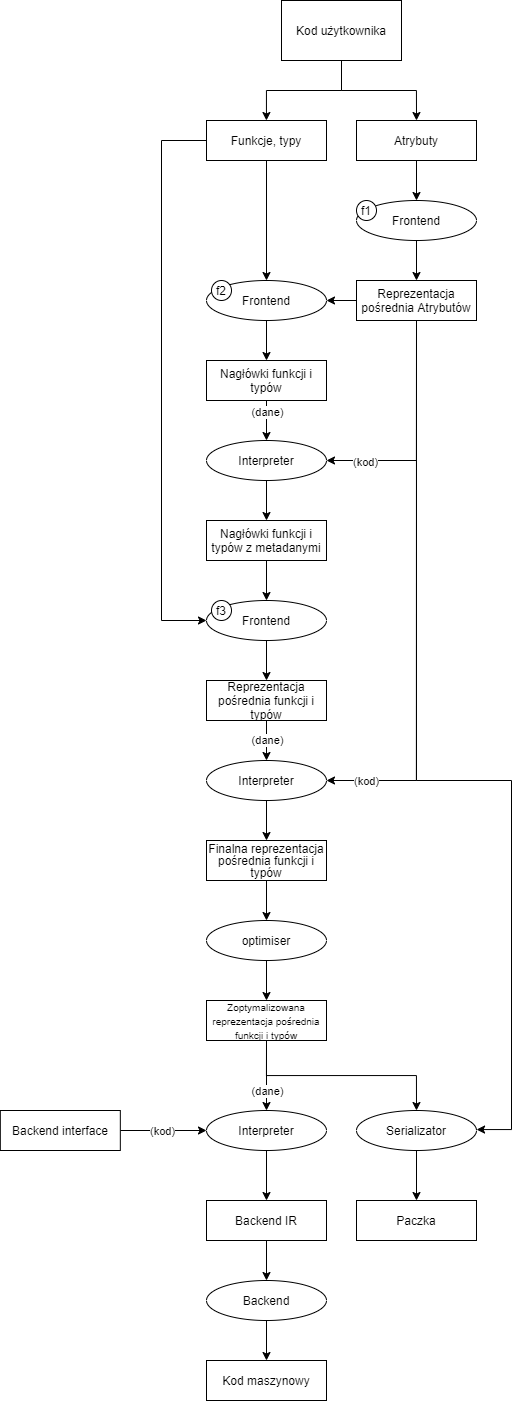
\includegraphics[scale=0.8]{img/compilation_process.png}
\caption{diagram procesu kompilacji języka C-=-1}
\centering
\end{figure}
\subsection{Front-end}
Front-end kompilatora C-=-1 jest odpowiedzialny za interakcje z tekstem kodu źródłowego. Rysunek 1 przedstawia diagram procesu kompilacji. Front-end gra w nim kluczową rolę w początkowych fazach, przetwarzając zawartość plików źródłowych. Sposób w który źródła są odczytywane oraz analizowane jest opisany w rozdziale 4.2.1.
Zrealizowanie tego procesu wymagało aby ten komponent kompilatora potrafił funkcjonować w różnych trybach w zależności od obecnie wykonywanego kroku. Ponadto, ponieważ w C-=-1, w przeciwieństwie do C++, kolejność deklaracji nie ma znaczenia, front-end musiał radzić sobie z zależnościami kołowymi. Ogół działania front-endu jest opisany w rozdziale 4.2.2.
\subsubsection{Parser}
Do parsowania tekstu wejściowego, użyto generatora parserów Rose [10]. Jest to narzędzie bazujące na Antlr, które znacząco ułatwia manipulowanie drzewem składniowym (ang. AST). Te dodatkowe możliwości są wykorzystywane przy przetwarzaniu szablonów (rozdział 4.2.5).
Kompilator trzyma w pamięci tylko jedno drzewo rozkładu na raz, co oznacza że każdy plik jest wczytywany wielokrotnie. Ta decyzja ma ograniczyć ilość zużywanej w danym momencie pamięci operacyjnej.
W celu analizy tekstu wejściowego użyto wizytatorów. Jest to typowy wzorzec projektowy w 
\subsubsection{Fazy przetwarzania plików źródłowych}

\subsubsection{Zarządzanie zależnościami}

\subsubsection{Import symboli zewnętrznych}

\subsubsection{Reprezentacja pośrednia}
Reprezentacja pośrednia jest istotnym elementem języka, na którym opiera się meta-programowanie w C-=-1. W związku z czym, każda jej część jest udokumentowana w załączniku 1. Wewnątrz kompilatora, reprezentacja pośrednia jest przechowywana w ramach struktur danych interpretera (rozdział 4.3.1), aby umożliwić interakcję z interpretowanym kodem.
Ponieważ użytkownik C-=-1 ma operować na CIR (C-=-1 Intermidiate Representation), jej struktura jest bliska językowi który reprezentuje. Poza dodaniem specjalnych typów instrukcji, struktura CIR jest niemal identyczna do C-=-1. Takie podejście ma zarówno wady i zalety. 
Z jednej strony sprawia ono, że błędy w kompilatorze są łatwiejsze, oraz front-end jest łatwiejszy do implementacji. Przez podobieństwo do kodu źródłowego sprawia że różnice względem poprawnego rezultatu są dużo bardziej oczywiste od bardziej abstrakcyjnych reprezentacji.
Taka reprezentacja jest jednak dużo trudniejsza do interpretowania. W przeciwieństwie do języków takich jak CIL (Common Intermediate Language) [11], CIR nie operuje abstrakcyjnej maszynie stosowej. Szczegółowy opis działania interpretera znajduje się w rozdziale 4.3.
Główne różnice w strukturze między C-=-1 a CIR polegają na bardziej dosłownym wyrażeniu programu. W reprezentacji pośredniej, wszystkie odniesienia są w pełni kwalifikowane nazwą paczki i przestrzenią nazw. Finalizatory są wywoływane wprost, używając specjalnej instrukcji. Zamiast rozwiązywania przeciążeń funkcji, CIR odnosi się do konkretnego przeciążenia przez unikatowy identyfikator.
\subsubsection{Szablony}

\subsection{Interpreter}
Interpreter C-=-1 operuje na reprezentacji pośredniej tego języka (rozdział 4.2.5).
\subsubsection{Reprezentacja obiektów}
\subsubsection{Wykonanie kodu}
\subsubsection{Funkcje specjalne}
\subsubsection{Referencje do obiektów C++}
\subsection{Serializator}
\subsection{Backend Interface}
Odpowiedzialnością interfejsu back-endu jest przetłumaczenie CIR na LIR. Na tym etapie kompilacji, cała reprezentacja pośrednia C-=-1 jest przechowywana w ramach struktur danych interpretera. Stworzyło to okazję do napisania części kompilatora w języku docelowym.
To rozwiązanie zapewniło bezpieczeństwo typów w tej części kodu oraz ułatwiło rozwój C-=-1. Tworzenie kompilatora w języku docelowym jest typowym w konstrukcji tego typu narzędzi. Program tak skonstruowany nazywają się „Bootstrapping Compiler” [12]. 
Implementacja tej części kompilatora w C-=-1 ułatwiła rozwój tego języka. Jedną z głównych zalet narzędzia skonstruowanego w ten sposób jest istnienie dużego projektu w języku docelowym. Wymusza to szybszy rozwój języka oraz umożliwia znajdowanie błędów w kompilatorze.
\subsubsection{Funkcje eksponowane przez kompilator}
Używając mechanizmów, opisanych w rozdziałach 4.3.3 oraz 4.3.4, interfejsowi backendu narzędzie do budowy LIR zdefiniowane w LLVM. Za jego pomocą może generować reprezentacje pośrednią LLVM.
W ramach biblioteki backendu, istnieje cała gama funkcji oraz typów używanych do emitowania reprezentacji pośredniej. Duża ich część została wyeksponowana interfejsowi backendu.
\subsubsection{Implementacja interfejsu backendu}
Razem z plikiem wykonywalnym kompilatora, dystrybuowany jest kod źródłowy paczki, zawierającej interfejs backendu. Przed kompilacją kodu użytkownika, kompilator wczytuje ten moduł. Zaletą tego rozwiązania jest możliwość wymiany tego komponentu, bez rekompilacji całego narzędzia.
Po załadowaniu tej paczki, kompilator szuka w niej zestawu funkcji createTranslator która służy jako punkt wejścia dla interfejsu. Ma ona za zadanie zainicjować paczkę oraz zwrócić implementacje interfejsu ITranslator. Zostanie ona użyta do generowania LIR dla poszczególnych struktur języka.

\subsection{Backend}
Do generowania kodu maszynowego została wykorzystana biblioteka LLVM.
\subsection{Biblioteka standardowa}

\subsection{Narzędzia dodatkowe}

\subsubsection{Tryb interaktywny}

\subsubsection{Debugger}

\subsubsection{Wtyczka do VS code}
\subsection{Wyzwania}
Generyki są zależne od kontekstu
Specjalne operatory nameof typeof etc
odchudzenie kompilatora przez trzymanie metadanych o funkcjach jako runtime value i funkcje do dostępu do tego jako klucz-wartość
\section{Porównanie z innymi językami}
Ponieważ C-=-1 jest językiem badawczym, nie można go porównywać z językami stosowanymi w przemyśle pod względem wygody użycia. Warto jednak przeanalizować, w jaki sposób zaproponowane mechanizmy wpływają na jego użyteczność.
\subsection{Wsparcie dla paradygmatów programowania}
Teoretycznie niemalże w każdym języku da się programować w każdym paradygmacie. Jednak w zależności od struktury tego języka, może być to zadanie prostsze lub trudniejsze. 
\subsubsection{Aspect oriented programming}
Nieoczekiwanym skutkiem zaproponowanych mechanizmów jest wsparcie dla AOP.
\subsubsection{Obiektowe}
C-=-1 został zaprojektowany z myślą o wsparciu stylu obiektowego. Użytkownik może deklarować typy, metody oraz interfejsy. W przeciwieństwie do C++ czy C\#, w C-=-1 nie ma jednak koncepcji dziedziczenia między konkretnymi klasami.

Klasy i interfejsy mogą implementować inne interfejsy. To jest jedyny mechanizm dynamicznego polimorfizmu w C-=-1. Ta decyzja została podjęta częściowo w celu uproszczenia języka, a częściowo ponieważ dziedziczenie między konkretnymi klasami jest uważane za złą praktykę.

\subsection{Walidacja kodu}
Podstawowym celem C-=-1 było zbadanie możliwości statycznej walidacji kodu, używając zaproponowanych mechanizmów metaprogramowania.
W kolejnych rozdziałach omówione zostaną przykładowe analizatory, które zostały zaimplementowane w ramach biblioteki standardowej, bądź których implementacja jest możliwa.
Ma to zademonstrować praktyczne aplikacje udostępnienia programiście modelu semantycznego tworzonego programu.



\subsubsection{Atrybut noDiscard}
\label{no_discard}

Atrybut \lstinline{noDiscard} służy do zapewnienia, że wynik funkcji nie zostanie zgnorowany.
Tego typu adnotacja istnieje w C++ od wersji 17.
Ma on na celu wyeliminować błędy takie jak ignorowanie kodu błędu, czy niepoprawne wywołanie funkcji o mylącej nazwie.

W C-=-1, w przeciwieństwie do większości języków niskiego poziomu, stworzenie analizatora który zapewnia taką walidację jest trywialne.
Listing \ref{lst:noDiscardCm1} zawiera kod atrybutu \lstinline{noDiscard} z biblioteki standardowej C-=-1.
Na linii 4 deklaruje on specjalną funkcję \lstinline{onCall} (specjalne funkcje atrybutów zostały opisane w rozdziale \ref{Attributes_cm1}), która reaguje na wywołania funkcji do której został zaaplikowany.

Wewnątrz tego podprogramu, atrybut sprawdza czy bezpośrednim rodzicem tego wyrażenia jest wyrażenie czy instrukcja.
Jeśli jest nim instrukcja, oznacza to że wynik wywołania jest ignorowany i trzeba zgłosić błąd, używając funkcji \lstinline{raiseError}.
W przeciwnym wypadku żadne akcje nie są konieczne.

Listing \ref{lst:noDiscardUsageCm1} demonstruje zastosowanie atrybut \lstinline{noDiscard}.
Zignorowanie wartości zwracanej przez funkcję oznaczoną tą odnotacją, tak jak na linii 5, powoduje zgłoszenie błędu o kodzie i komunikacie zgodnym z linią 7 listingu \ref{lst:noDiscardCm1}.
Ponadto, kompilator otrzymuje wskazanie do pliku źródłowego na punkt, który wywołał ten błąd.
Ta informacja może być potem użyta do zaprezentowania programiście dokładniejszej diagnostyki, bądź do podkreślenia kodu w zintegrowanym środowisku programistycznym (rozdział \ref{IDE_integration}).

Ten przykład dobrze ilustruje, że mając dostęp do modelu semantycznego programu, implementajca niektórych typów walidacji staje się trywialna.
W większości języków programowania taka analiza wymaga modyfikacji kompilatora albo zewnętrznego narzędzia.

\begin{minipage}{\linewidth}
  
  \begin{lstlisting}[
    numbers=left,
    firstnumber=0,
    caption={Atrybut noDiscard w C-=-1},
    aboveskip=0pt,
    label={lst:noDiscardCm1}
    ]
public att<function> NoDiscard
{
  public fn attach(f: functionDescriptor)
  {}
  public fn onCall(call: functionCallExpression*)
  {
  if(call._parentStatment != null<IInstruction>())
    raiseError(
      &(call._pointerToSource), 
      "Return value of a no-discard function is not used",
      123
    );
  }
}
\end{lstlisting}
\end{minipage}


\begin{minipage}{\linewidth}
  
  \begin{lstlisting}[
    numbers=left,
    firstnumber=0,
    caption={Przykład użycia atrybut noDiscard w C-=-1},
    aboveskip=0pt,
    label={lst:noDiscardUsageCm1}
    ]
[noDiscard()]
fn noDiscardFunction() -> usize;

fn main() -> usize
{
  noDiscardFunction(); // error 123: Return value of
                       // a no-discard function is not use
  let x = noDiscardFunction();     // ok
  let y = x + noDiscardFunction(); // ok
  return noDiscardFunction();      // ok
}
\end{lstlisting}
\end{minipage}

\subsubsection{Atrybut const}
\label{const}

Bardziej złożonym przykładem analizatora, jest atrybut \lstinline{const}.
Odpowiada on modyfiaktorowi \lstinline{const} z języka C++.
Zaaplikowanie go do typu oznacza, że do jego instancja jest niemodyfikowalna.
Każda próba modyfikacji, po zainicjalizowaniu, jest błędem.

W obecnym stanie kompilatora oraz języka, możliwa jest implementacja części tej funkcjonalności.
Pełne wsparcie dla tego modyfikatora, przy użyciu atrybutu, wymaga od C-=-1 następujących właściwości:
\begin{enumerate}
  \item \label{prop:Attribute_function_overloading} Atrybuty są brane pod uwagę w trakcie wyboru przeciążenia funkcji
  \item \label{prop:Generic_adnotations} Istnieje sposób na modyfikowanie zachowania zmiennych, pól i parametrów w generykach, przy tworzeniu ich instancji
  \item \label{prop:Reference_adnotations} Przy aplikowaniu atrybutu do zmiennej typu referencyjnego, istnieje sposób na rozróżnienie między stałym wskazaniem a wskazaniem na stałą.
\end{enumerate}


\subsection{Generowanie kodu}

\subsubsection{Atrybut Flags}

\subsection{Testowanie kodu}

\subsection{Rozszerzalność języka}
\label{Language_extensibility}
Jedną z konsekwencji zaproponowanych mechanizmów jest możliwość rozszerzania języka bez modyfikacji kompilatora.
Oznacza to że pewne elementy składni, obecne w innych językach, stają się zbędnę w C-=-1.
\subsubsection{Symbole zewnętrzne}
Większość języków programowania zawiera mechanizm umożliwiający import symboli zewnętrznych.
Mogą one pochodzić z kodu napisanego w innym języku lub z już skompilowanej biblioteki.

W wypadku C/C++, wymaga to użycia słowa \lstinline{external}, do zdefiniowania symbolu zewnętrznego oraz przekazania odpowiedniego argumentu do linkera.
W C-=-1 ten sam rezultat można osiągnąć, przypisując funkcji odpowiednie metadane, które potem zostaną odczytane przez interfejs backendu.
Wbudowana wersja tego programu obsługuje wczytywanie definicji funkcji z plików lib oraz zastępowanie jej ciała kodem LLVM.

Listing \ref{lst:replaceWithLLVMAttribute} przedstawia atrybut \lstinline{replaceWithLLVMIR} z biblioteki standardowej C-=-1. 
Pobiera on kod LLVMIR z pliku wskazanego przez użytkownika, a następnie ustawia w definicji wybranej funkcji zmienną "llvm-representation".
Backend interface może potem odczytać tą wartość i wykorzystać ją do wygenerowania kodu dla backendu.


\begin{lstlisting}[
    numbers=left,
    firstnumber=0,
    caption={Atrybut zastępujący ciało funkcji kodem LLVM},
    aboveskip=0pt,
    label={lst:replaceWithLLVMAttribute}
]
public att<function> ReplaceWithLLVMIR
{
  private _filename: string;
  private _nameOftypeToReplace: string;
  private _nameToReplace: string;

  public fn construct(
    filename: string,
    nameOfTypeToReplace: string,
    nameToReplace: string)
  {
    self._filename = filename;
    self._nameOftypeToReplace = nameOfTypeToReplace;
    self._nameToReplace = nameToReplace
  }

  public fn attach(f: functionDescriptor)
  {
    let ir = read_all_file(self._filename);
    ir = ir.replace("$" + self._nameOftypeToReplace, self._nameToReplace);
    f.store("llvm-representation", ir);
  }
}

\end{lstlisting}

\section{Wyzwania}

\subsection{Funkcje generyczne z ograniczeniami}

Funkcje mogą być wykluczane w trakcie uruchomienia lub kompilacji. Jeśli generyk takiej funkcji zostanie stworzony z typem dalej ograniczającym wykonywalność tej funkcji, ona może być wykonywalna nigdy.

\subsection{Operator new}

Operator \mintinline{Cpp}{new} w C-=-1, tak jak w C++ służy do dynamicznej alokacji pamięci na stercie.


\subsection{Wybór przeciążenia funkcji}
To czy funkcja jest wykonywalna w czasie kompilacji albo uruchomienia można ustalić bardzo późno w trakcie budowy modelu semantycznego.

\subsection{Wyrażenia literałowe}

Wyrażenie literałowe przedstawia stałą wartość.
Na przykład w języku C++ \mintinline{CPP}{int a = 4;} deklaruje i inicjalizuje zmienną a literałem 4.
Wyrażenia lietrałowe mogą reprezentować stałe różnych typów wbudowanych 

\subsection{Integracja z back-endem}
Przy pierwszym podejściu do budowy reprezentacji pośredniej, użyto dedykowanych struktur danych. Było to podejście najbardziej naturalne i dające najwięcej bezpieczeństwa dzięki silnemu typowaniu. Wszystkie struktury danych opisane w rozdziale \ref{reprezentacja_posrednia} miały powiązane ze sobą klasy C++.


To podejście tworzy jednak duży problem. Reprezentacja pośrednia musi zostać wyeksponowana użytkownikowi. Ponieważ nie istniała możliwość stworzenia binarnego interfejsu między kompilatorem a interpretowanym kodem, struktury danych CIR musiały być dodatkowo reprezentowane za pomocą struktur danych interpretera.


Użytkownik może dokonywać modyfikacji w CIR, co oznacza że może dojść do rozbieżności między strukturami danych interpretera a kompilatora. Utrzymywanie tych dwóch reprezentacji stanowiło poważne wyzwanie, dlatego postanowiono zmienić podejście. Użycie wyłącznie struktur danych interpretera do reprezentacji CIR usunęło ten problem, kosztem bezpieczeństwa kodu.


Ponieważ w nowym podejściu, z perspektywy C++ niemalże wszystkie obiekty miały ten sam typ, kompilator stracił możliwość statycznej weryfikacji kodu.
Aby zapewnić poprawność programu, koniecznym stało się dodawanie walidacji argumentów do wszystkich funkcji.

\subsection{Informacje dodatkowe o obiektach}
Na wczesnej fazie projektu koniecznym okazało się przechowywanie informacji które nie zostały uwzględnione w modelu semantycznym.
Potrzeba ta powstała przy implementacji operatora \mintinline{Cpp}{sizeof}.
Ponieważ rozmiar obiektów jest ustalany dopiero przez LLVM, koniecznym stało się zastąpienie kodu funkcji, reprezentacją pośrednią backendu.

Rozwiązanie tego problemu wymaga wzięcia pod uwagę kilku istotnych aspektów.
Zostały one opisane w rozdziałach \ref{frontend_responsibility}, \ref{compiler_extensibility} oraz \ref{frontend_backend_complexity}.
Rozdziały \ref{original_solution} i \ref{final_solution}

\subsubsection{Oryginalne rozwiązanie}\label{original_solution}

Naturalnym podejściem do problemu, było zawarcie metadanych o obiekcie, wewnątrz jego definicji.
W ten sposób frontend miał do nich łatwy dostęp.

\subsubsection{Zakres odpowiedzialności frontendu} \label{frontend_responsibility}

\subsubsection{Rozszerzalność kompilatora}\label{compiler_extensibility}

\subsubsection{Złożoność granicy frontend-backend interface} \label{frontend_backend_complexity}

\subsubsection{Ostateczne rozwiązanie}\label{final_solution}
Po przeanalizowaniu rozwiązania z rozdziału \ref{original_solution} pod kątem problemów wymienionych w rozdziałach \ref{frontend_responsibility}, \ref{compiler_extensibility} oraz \ref{frontend_backend_complexity}, postanowiono radykalnie zmienić podejście.
Zamiast definiować metadane obiektów po stronie struktur danych frontendu, postanowiono zdefiniować interfejs umożliwiający zapis i metadanych o elementach modelu semantycznego. 
Listing \ref{lst:IMetadataHolder} zawiera jego deklarację.
Metody store i get zdefiniowane na liniach 2 i 3 umożliwiają zapis i odczyt metadanych.

Ten interfejs został zaimplementowany po stronie frontendu.
Ponieważ w tym kontekście sprawdzanie typów jest opcjonalne, nie wymagało to wprowadzania dodatkowych mechanizmów do języka takich jak \mintinline{Cpp}{std::any}.

W porównaniu z rozwiązaniem z oryginalny rozwiązaniem, to podejście znacząco zmniejsza granice między frontendem a interfejsem backendu.
Ponadto, podział odpowiedzialności pomiędzy tymi komponentami jest dużo bardziej logiczny.
Frontend nie wiedzieć o tym jakie informacje są potrzebne przy kompilacji.
Ponadto, ponieważ metadane które mogą być przechowywane nie są zdefiniowane odgórnie, znacząco zwiększa też rozszerzalność kompilatora.

\begin{lstlisting}[
    language=Cm1,
    numbers=left,
    firstnumber=0,
    caption={Interfejs obiektu przechowującego metadane},
    aboveskip=0pt,
    label={lst:IMetadataHolder}
]
class IMetadataHolder
{
    public fn store<T>(key: string, value: T);
    public fn get<T>(key: string) -> T;
    public fn has(key: string) -> bool;
}

class functionDescriptor : IMetadataHolder;
class typeDescriptor : IMetadataHolder;
class fieldDescriptor : IMetadataHolder;
class variableDescriptor : IMetadataHolder;
\end{lstlisting}
\section{Wnioski}

C-=-1, z oczywistych powodów, pod wieloma wzgęldami jest gorszy od istniejących rozwiązań.
Wiele udogodnień, traktowanych już jako standard, takich jak dedukcja parametrów generycznych czy semantyka przenoszenia nie zostało zaimplementowanych z powodu braku czasu.
Ponadto wsparcie dla C-=-1 jest minimalne: nie istnieje edytor, który koloruje jego składnie, a kompilator oferuje w najlepszym wypadku bardzo podstawową diagnostykę.
Jego celem nie było jednak zastąpić C++, Rust czy C\#, a zbadać jak priorytetyzacja wsparcia dla statycznego metaprogramowania wpływa na język oraz pisany w nim kod. 
Pod tym względem, C-=-1 można uznać za sukces.

Wiele aspektów tego języka, zostało niestety omówione wyłącznie na poziomie teoretycznym, ze względu na brak wsparcia kompilatora.
Stworzenie nowego języka programowania jest zadaniem dużo bardziej złożonym i czasochłonnym niż zakładano na początku tej pracy.
Z tego powodu, zabrakło czasu, aby zrealizować projekt C-=-1 w pełni.


\subsection{Kategoryzacja języka}

C-=-1 od samego początku był definiowany jako kompilowany język programowania ze wsparciem dla statycznego metaprogramowania i wykonywania kodu w czasie kompilacji.
Oryginalny projekt implementacji zakładał więc, że kompilator będzie zawierał w sobie moduł interpretujacy reprezentację pośrednią programu.
Po wykonaniu transformacji na kodzie użytkownika kompilator miał przejąć kontrolę i dokonać kompilacji do kodu maszynowego.

Jednak w wyniku zmian opisanych w rozdziale \ref{Backend_Interface}, kompilacja do kodu maszynowego została zaimplementowana w interpretowanym C-=-1.
Oznacza to, że kompilator składa się wyłącznie z frontendu oraz środowiska uruchomieniowego które, udostępnia intefejs biblioteki llvm.
Z tego powodu, w ogólnym przypadku, C-=-1 można zaklasyfikować jako silnie typowany język interpretowany.

Należy jednak pamiętać, że ten język zawiera w sobie rozróżnienie między kodem wykonywalnym w czasie uruchomienia a kompilacji.
Ponadto, jego projekt zawiera semantykę typową dla języków kompilowanych: jawną alokację obiektów na stercie, ręczne zarządzanie pamięcią oraz wskazania. 
Ten aspekt został opisany w rozdziale \ref{Language_desig}.
Tak więc najlepszym sposobem na zkategoryzowanie C-=-1 jest uznanie go za hybrydę pomiędzy językiem kompilowanym a interpretowanym.


\subsection{Rozszerzalność języka}

Umożliwienie programiście modyfikowanie kodu oraz tworzenie własnych adnotacji sprawia, że język można bardzo łatwo rozszerzyć o nowe mechanizmy.
W rozdziale \ref{Language_extensibility} opisano przykłady składni nie wspieranej przez C-=-1, a którą można dodać przy użyciu proponowanego mechanizmu atrybutów.

Wykorzystując go, programista może zawęzić zbiór programów akceptowanych przez kompilator, przy użyciu analizy statycznej.
W rozdziałach \ref{no_discard} oraz \ref{const} przedstawiono przykłady adnotacji istniejących w C++ jako część języka, które można dodać do C-=-1.
Po dodaniu mechanizmu wyjątków, trywialną będzie też implementacja atrybutu \lstinline{noexcept}, oznaczającego funkcje która nigdy nie rzuca.

\subsection{Możliwa krytyka}

Zaproponowane podejście niesie ze sobą pewne wady.
Być możne najpoważniejszą z nich jest utrudniony rozwój kompilatora.
Ponieważ model programu musi edytowalny przez interpretowany kod, należy go zbudować ze struktur danych interpretera.
Dokładne uzasadnienie i opis implementacji znajduje się w rozdziale \ref{backend_integration}.
Opisane tam wyzwania stanowią argument przeciwko konstruowaniu języków programowania w ten sposób. 
Chwilowo nie ma alternatywnej implementacji, która zachowuje silne typowanie w kodzie kompilatora.

Inny problem, dotyczy samej konstrukcji języka.
Zaproponowane w tej pracy mechanizmy metaprogramistyczne, mogą prowadzić do zwiększenia poziomu złożoności tworzonego kodu.
Ponieważ atrybuty w C-=-1 mogą nadpisywać kod użytkownika, nadużycie tego mechanizmu może prowadzić do trudno przewidywalnego zachowania.
Zasadność tej krytyki powinna być tematem przyszłych badań.

%todo: opisać problem z systemem typów ad-hoc


\newpage % Rozdziały zaczynamy od nowej strony
\section{Summatio}          % Można też pisać rozdziały w jednym pliku.


%--------------------------------------------
% Literatura
%--------------------------------------------
\cleardoublepage % Zaczynamy od nieparzystej strony
\printbibliography

%--------------------------------------------
% Spisy (opcjonalne)
%--------------------------------------------
\newpage
\pagestyle{plain}

% Wykaz symboli i skrótów.
% Pamiętaj, żeby posortować symbole alfabetycznie
% we własnym zakresie. Ponieważ mało kto używa takiego wykazu,
% uznałem, że robienie automatycznie sortowanej listy
% na poziomie LaTeXa to za duży overkill.
% Makro \acronymlist generuje właściwy tytuł sekcji,
% w zależności od języka.
% Makro \acronym dodaje skrót/symbol do listy,
% zapewniając podstawowe formatowanie.
% //AB
\vspace{0.8cm}
\acronymlist
\acronym{EiTI}{Wydział Elektroniki i Technik Informacyjnych}
\acronym{PW}{Politechnika Warszawska}
\acronym{WEIRD}{ang. \emph{Western, Educated, Industrialized, Rich and Democratic}}

\listoffigurestoc     % Spis rysunków.
\vspace{1cm}          % vertical space
\listoftablestoc      % Spis tabel.
\vspace{1cm}          % vertical space
\listofappendicestoc  % Spis załączników

% Załączniki
\newpage
\appendix{Nazwa załącznika 1}


\newpage
\appendix{Nazwa załącznika 2}


% Używając powyższych spisów jako szablonu,
% możesz tu dodać swój własny wykaz bądź listę,
% np. spis algorytmów.

\end{document} % Dobranoc.
